\usepackage[italian]{babel}
\usepackage[utf8]{inputenc}
\usepackage{pgf}
\usepackage{verbatim}
\usepackage{inconsolata}
\usepackage{listings}
\lstset{language=C, frame=single,
  basicstyle=\scriptsize\ttfamily,
  numbers=left, numberstyle=\tiny\color{gray},
   numbersep=5pt, fancyvrb=true
}

\usefonttheme{professionalfonts} % using non standard fonts for beamer
\usefonttheme{serif} % default family is serif
% \usepackage{fontspec}
% \setmainfont{Palatino}

\usepackage{url}
\usepackage{xmpmulti}
% \usepackage{euler}
\usepackage[T1]{fontenc}
\pdfpagebox5
\immediate\write18{sh ./vc}
\input{vc}

\author{Gianluca Della Vedova}
\title{Elementi di Bioinformatica}
\institute{Univ. Milano--Bicocca\\
  \texttt{http://gianluca.dellavedova.org}}
\date{\today, {\tiny revisione \VCRevision}}
%\pgfdeclareimage[height=1cm]{university-logo}{logounimib}
%\logo{\pgfuseimage{university-logo}}



% If you wish to uncover everything in a step-wise fashion, uncomment
% the following command:
\beamerdefaultoverlayspecification{<+->}

\graphicspath{{figures/}}


\begin{document}
\begin{frame}
  \titlepage
\end{frame}


\begin{frame}\frametitle{Gianluca Della Vedova}
\begin{itemize}
\item
Elementi di Bioinformatica
\item
Ufficio U14-2041
\item
\url{http://gianluca.dellavedova.org}
\item
\url{http://elearning.unimib.it/course/view.php?id=4071}
\item
\url{gianluca.dellavedova@unimib.it}
\end{itemize}
\end{frame}

\begin{frame}[fragile]
\frametitle{Notazione}
\begin{itemize}
\item
\alert{simbolo}: $T[i]$\\
\item
\alert{stringa}: $T[1]T[2]\cdots T[l]$\\
\item
\alert{sottostringa}: $T[i:j]$\\
\item
\alert{prefisso}: $T[:j]=T[1:j]$\\
\item
\alert{suffisso}: $T[i:]=T[i:|T|]$
\item
\alert{concatenazione}: $T_{1}\cdot T_{2} = T_{1}T_{2}$
\end{itemize}
\end{frame}


\begin{frame}[fragile]
\frametitle{Pattern Matching}
\begin{block}{Problema}
\alert{Input}: testo $T=T[1]\cdots T[n]$, pattern $P=P[1]\cdots P[m]$, alfabeto $\Sigma$\\
\alert{Goal}: trovare \emph{tutte} le occorrenze di $P$ in $T$\\
\alert{Goal}: trovare tutti gli $i$ tale che $T[i]\cdots T[i+m-1]=P$
\end{block}
\begin{block}{Algoritmo banale}
\alert{Tempo}: $O(nm)$
\end{block}
\begin{block}{Lower bound}
\alert{Tempo}: $O(n+m)$
\end{block}
\end{frame}

\begin{frame}
\frametitle{Bit-parallel}
\begin{block}{Algoritmi seminumerici}
\begin{itemize}
\item
$25$
\item
$25=00011001$
\item
$25=00011001=$FFFTTFFT
\end{itemize}
\end{block}
\begin{block}{Operazioni bit-level}
\alert{Or}: $x\lor y$, \alert{And}: $x\land y$, \alert{Xor}: $x\oplus y$\\
\alert{Left Shift}: $x << k$, \alert{Right Shift}: $x >> k$,
\begin{itemize}
\item
Tutte bitwise
\item
Tutte in hardware
\end{itemize}
\end{block}
\end{frame}

\begin{frame}
\frametitle{D\"om\"olki / Baeza-Yates, Gonnet}
\begin{block}{Matrice $M$}
$M(i,j)=1$ sse $P[:i]=T[j-i+1:j]$\\
$0\le i\le m$, $0\le j\le n$
\end{block}
\begin{block}{Occorrenza di $P$ in $T$}
$M(m,j)=1$
\end{block}
\begin{itemize}
\item
$M(0,\cdot)=1$, $M(\cdot,0)=0$
\item
\alert{$M(i,j)=1$} sse $M(i-1, j-1)=1$ AND $P[i]=T[j]$
\end{itemize}
\end{frame}

\begin{frame}
\frametitle{Esempio}
\begin{block}{Esempio}
$T$=abracadabra\\
$P$=abr
\end{block}

\begin{center}
\begin{tabular}[l]{ll}
%\hline{1}
10010101001\\
01000000100\\
00100000010&$\leftarrow$ \alert{occorrenze}\\%\hline
\end{tabular}
\end{center}

\begin{block}{Matrice $M$}
1 colonna = 1 numero
\end{block}
\end{frame}

\begin{frame}[fragile]
\frametitle{Colonne}
$U[\sigma]$ = array di bit dove $U[\sigma,i]=1$ sse $P[i]=\sigma$

\begin{block}{$C[j]$ da $C[j-1]$}
\begin{itemize}
\item
Right shift di $C[j-1]$
\item
$1$ in prima posizione
\item
AND con $U[T[j-1]]$
\item
\alert{w}: word size
\item
C[j] = ((C[j-1] >> 1) || (1 << (w-1))) \& U[T[j]];
\end{itemize}
\end{block}
\end{frame}

\begin{frame}[fragile]
\frametitle{Note}
\begin{itemize}
\item
Tempo $O(n)$ se $m\le w$
\item
Tempo $O(nm)$
\item
No condizioni
\item
$w<m\le 2w$?
\end{itemize}
\end{frame}

\begin{frame}[fragile]
\frametitle{Karp-Rabin}
\begin{block}{Alfabeto binario}
\begin{itemize}
\item
$H(S)=\sum_{i=1}^{|S|} 2^{i-1}H[i]$
\item
sliding window di ampiezza $m$ su $T$
\item
$H(T[i+1:i+m]) =$\\
$=\left(H(T[i:i+m-1]) - T[i] \right) / 2 + 2^{m-1}T[i+m-1]$
\item
operazioni su bit
\item
$T[i:i+m-1]=P \Leftrightarrow H(T[i:i+m-1])=H(P)$
\end{itemize}
\end{block}
\end{frame}

\begin{frame}[fragile]
\frametitle{Karp-Rabin: problema}
\begin{block}{Numeri troppo grandi}
\begin{itemize}
\item
Modello RAM: numeri $O(n+m)$
\item
mod $p$
\item
$H(T[i+1:i+m]) =$\\
$\left(\left(H(T[i:i+m-1]) - T[i] \right) / 2 + 2^{m-1}T[i+m] \right)\mod p$
\item \textbf{NO}
\item
$2^{m-1}T[i+m] \mod p$ calcolato iterativamente, $\mod p$ ad ogni passo
\end{itemize}
\end{block}
\end{frame}

\begin{frame}[fragile]
\frametitle{Karp-Rabin: falsi positivi}
\begin{block}{Possibili errori}
\begin{itemize}
\item
Falso positivo (FP): occorrenza non vera
\item
Falso negativo (FN): occorrenza non trovata
\item
$H(T[i:i+m-1])=H(P) \Leftrightarrow T[i:i+m-1]=P$
\item
$H(T[i:i+m-1])  \mod p = H(P)  \mod p$
$\Leftarrow T[i:i+m-1]=P$
\end{itemize}
\end{block}
\end{frame}


\begin{frame}[fragile]
\frametitle{Karp-Rabin: falsi positivi}
\begin{block}{Probabilità di errore}
$P[\#FP\ge 1] \le O(nm/I)$ se il numero primo $p$ è scelto fra tutti i primi $\le
I$
\end{block}

\begin{block}{Valori di $I$}
\begin{itemize}
\item
$I=n^{2}m \Rightarrow P[\#FP\ge 1] \le 2.54/n$
\item
$I=nm^{2}  \Rightarrow P[\#FP\ge 1] \in O(1/m)$
\end{itemize}
\end{block}

\begin{block}{Abbassare probabilità di errore}
Scegliere $k$ primi casuali (indipendenti senza ripetizioni), cambiare primo
dopo ogni FP
\end{block}
\end{frame}

\begin{frame}[fragile]
\frametitle{Las Vegas vs.
  Monte Carlo}
\begin{block}{Classificazione algoritmi probabilistici}
\begin{itemize}
\item
Las Vegas:
\begin{itemize}
\item
Sempre corretto
\item
Forse non in tempo polinomiale
\item
Quicksort con pivot random
\end{itemize}
\item
Monte Carlo:
\begin{itemize}
\item
Sempre tempo polinomiale
\item
Forse non corretto
\item
Karp-Rabin
\end{itemize}
\end{itemize}
\end{block}
\end{frame}


\begin{frame}[fragile]
\frametitle{Controllo falsi positivi}
$L$: posizioni iniziali in $T$ delle occorrenze
\begin{block}{Run}
sequenza $\langle l_{1}, \ldots, l_{k}\rangle$ di posizioni in $L$ distanti al
massimo $m/2$
\end{block}

\begin{itemize}
\item
$d=l_{2}-l_{1}$
\item
$P$ semiperiodico con periodo $d$
\item
$P=\alpha\beta^{k-1}$, $\alpha$ suffisso di $\beta$
\item
ogni run occupa $\ge n$ caratteri di $T$
\item
ogni carattere  di $T$ è in max $2$ run
\end{itemize}
\end{frame}


\begin{frame}[fragile]
\frametitle{Trie}
\begin{columns}
\begin{column}{0.6\textwidth}
\begin{block}{Trie}
\begin{itemize}
\item
Albero
\item
Query: parola $\in$ dizionario
\item
archi etichettati
\item
Percorso radice-foglia = parola
\end{itemize}
\end{block}
\begin{block}{Dizionario}
ABRACADABRA\\
ARRAY\\
\uncover<3->{\alert{ABRA}}
\end{block}
\end{column}
\begin{column}{0.4\textwidth}
\begin{center}
\onslide<2-3>{\includegraphics[width=\textwidth]{trie1}}
%\onslide<4->{\includegraphics[width=\textwidth]{trie3}}
\end{center}
\end{column}
\end{columns}
\end{frame}

\begin{frame}[fragile]
\frametitle{Trie}
\begin{columns}
\begin{column}{0.6\textwidth}
\begin{block}{Terminatore}
\$ non appartiene all'alfabeto
\end{block}
\onslide<2->{\begin{block}{Dizionario}
ABRACADABRA\$\\
ARRAY\$\\
ABRA\$
\end{block}}
\end{column}
\begin{column}{0.4\textwidth}
\begin{center}
\onslide<3->{\includegraphics[width=\textwidth]{trie4}}
\end{center}
\end{column}
\end{columns}
\end{frame}

\begin{frame}[fragile]
\frametitle{Suffix tree}
\begin{columns}
\begin{column}{0.5\textwidth}
\begin{block}{Definizione}
\begin{itemize}[<+->]
% \item
% Testo $T$
\item
Trie compatto di tutti i suffissi di $T\$$
\item
Le etichette degli archi uscenti da $x$ iniziano con simboli diversi
\item
suffissi $\Leftrightarrow$ percorso radice-foglia
\end{itemize}
\end{block}
\end{column}
\begin{column}{0.5\textwidth}
\begin{center}
\uncover<4->{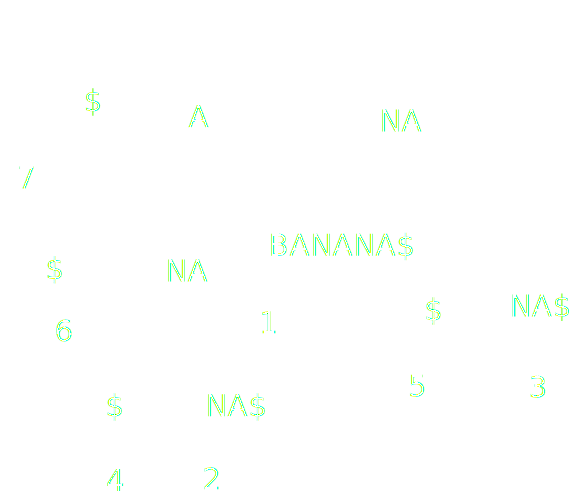
\includegraphics[width=\textwidth]{Suffix_tree_BANANA}

BANANA\$}
\end{center}
\end{column}
\end{columns}
\end{frame}

\begin{frame}[fragile]
\frametitle{Suffix tree 2: Definizione}
\begin{itemize}
\item
foglie etichettata con posizione inizio suffisso
\item
path-label$(x)$: concatenazione etichette
\item
string-depth$(x)$: lunghezza path-label$(x)$
\item
Pattern matching = visita
\end{itemize}
\begin{block}{Problemi}
\begin{itemize}[<+->]
\item
Spazio $O(n^{2})$
\item
Puntatori al testo (posizioni)
\item
Spazio $20n$ bytes
\end{itemize}
\end{block}
\end{frame}

\begin{frame}[fragile]
\frametitle{Suffix array}
\begin{block}{Definizione}
\begin{itemize}[<+->]
\item
Array dei suffissi in ordine lessicografico
\item
Posizioni iniziali del suffisso nell'array
\item
Spazio $4n$ bytes
\item
$Lcp[i]$: lunghezza prefisso comune $SA[i]$, $SA[i+1]$
\end{itemize}
\end{block}
\uncover<5->{\begin{block}{BANANA\$}
\begin{tabular}[l]{|c|l|l|l|l|l|l|l|}
\hline
$i$&0&1&2&3&4&5&6\\
$SA$&7&6&4&2&1&5&3\\
$Lcp$&0&1&3&0&0&2&-\\\hline
\end{tabular}}
\end{block}
\end{frame}

\begin{frame}[fragile]
\frametitle{Da Suffix tree a Suffix array}
\begin{columns}
\begin{column}{0.5\textwidth}
\begin{itemize}[<+->]
\item
Visita depth-first di $ST$
\item
archi uscenti di ogni nodo in ordine lessicografico
\item
$Lcp[i]$ = string-depth di $lca(i,i+1)$
\end{itemize}
\end{column}
\begin{column}{0.4\textwidth}
\begin{center}
\onslide<1->{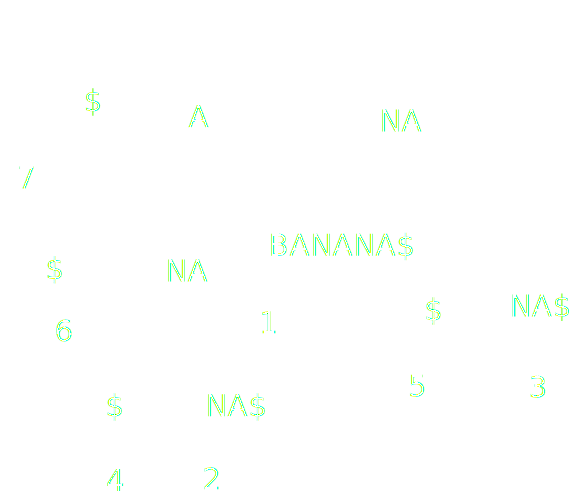
\includegraphics[width=\textwidth]{Suffix_tree_BANANA}}
%\onslide<4->{\includegraphics[width=\textwidth]{trie3}}
\end{center}
\end{column}
\end{columns}
\end{frame}

\begin{frame}[fragile]
\frametitle{Da Suffix array a Suffix tree}
\begin{columns}
\begin{column}{0.5\textwidth}
\begin{itemize}[<+->]
\item
$Lcp = 0$:  partizione $SA$
\item
corrispondono ai figli della radice
\item
ricorsione prendendo i numeri minimi
\end{itemize}
\begin{block}{BANANA\$}
\begin{tabular}[l]{|c|l|l|l|l|l|l|l|}
\hline
$i$&0&1&2&3&4&5&6\\
$SA$&7&6&4&2&1&5&3\\
$Lcp$&0&1&3&0&0&2&-\\\hline
\end{tabular}
\end{block}
\end{column}
\begin{column}{0.5\textwidth}
\begin{center}
\only<2>{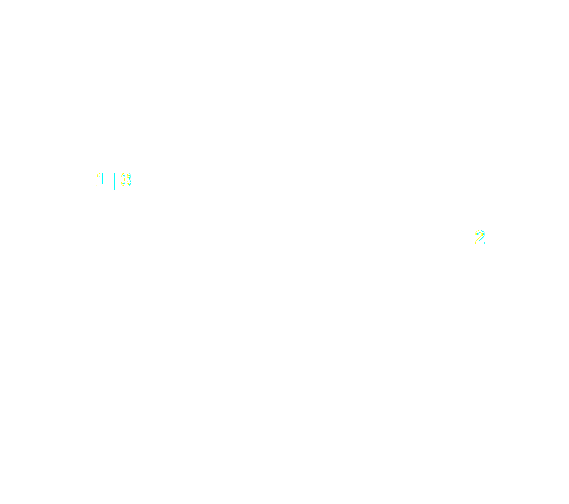
\includegraphics[width=\textwidth]{Suffix_tree_BANANA-level1}}
\only<3>{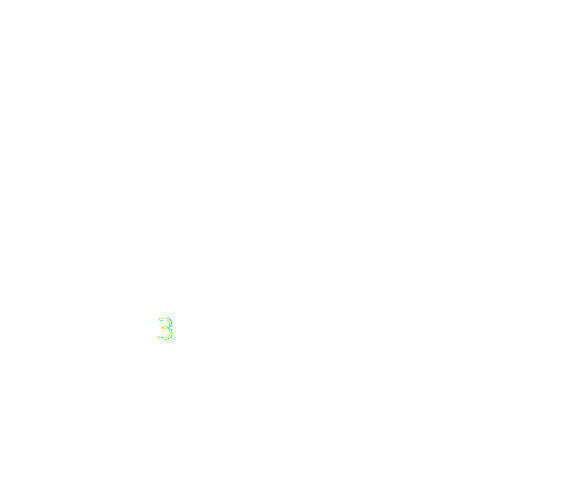
\includegraphics[width=\textwidth]{Suffix_tree_BANANA-level2}}
\only<4>{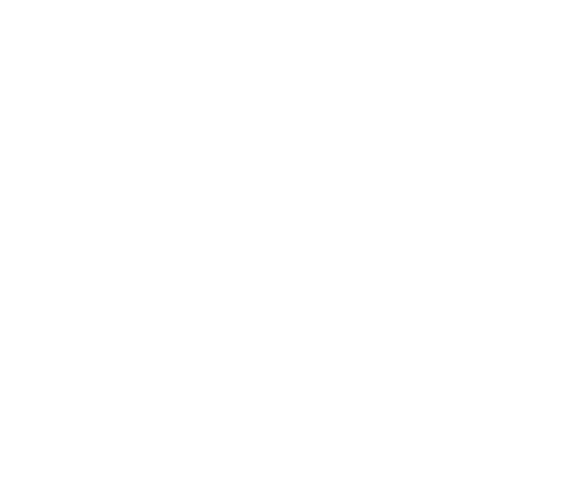
\includegraphics[width=\textwidth]{Suffix_tree_BANANA-level3}}
\only<5>{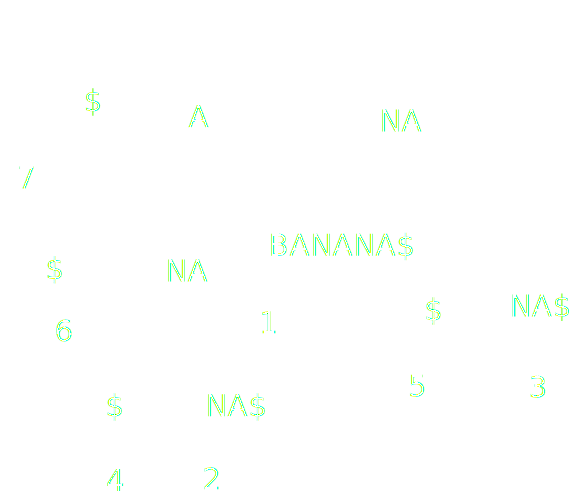
\includegraphics[width=\textwidth]{Suffix_tree_BANANA}}
\end{center}
\end{column}
\end{columns}
\end{frame}

\begin{frame}[fragile]
\frametitle{Pattern matching su suffix array}
\begin{block}{Occorrenza $P$ in $T$}
Suffissi di $T$ che iniziano con $P$
\end{block}
\begin{block}{Ricerca in $SA$}
\begin{itemize}
\item
Ricerca dicotomica
\item
Tempo $O(m \log m)$ -- caso pessimo
\item
Controllare tutto $P$ ad ogni iterazione
\item
$log_{2} m$ iterazioni
\end{itemize}
\end{block}
\end{frame}

\begin{frame}[fragile]
\frametitle{Acceleranti 1}
\begin{columns}
\begin{column}{0.5\textwidth}
\begin{itemize}
\item
Intervallo $SA(L, R)$ di $SA$
\item
Elemento mediano $M$
\item
Tutti i suffissi in $SA(L,R)$ iniziano con uno stesso prefisso lungo $Lcp(SA[L],
SA[R])$
\item
Non confrontare con i primi $Lcp(SA[L], SA[R])$ caratteri
\end{itemize}
\end{column}
\begin{column}{0.4\textwidth}
\begin{center}
\onslide<1->{\multiinclude[<+>][start=1,format=pdf,graphics={width=0.95\textwidth}]{figures/SA-pattern-matching1}}
%\onslide<4->{\includegraphics[width=\textwidth]{trie3}}
\end{center}
\end{column}
\end{columns}
\end{frame}

\begin{frame}[fragile]
\frametitle{Acceleranti 2}
\begin{columns}[T]
\begin{column}[T]{0.6\textwidth}
\begin{block}{$l$: $lcp(L,P)$; $r$: $Lcp(R,P)$}
\begin{enumerate}
\item
Caso 1: $l>r$
\only<3->{\begin{itemize}\item
$Lcp(L,M)>l$\only<4->{$\Rightarrow L\gets M$}
\only<5->{\item
$Lcp(L,M)<l$\only<6->{$\Rightarrow$\\ $R\gets M, r\gets Lcp(M,L)$}}
\only<7->{\item
  $Lcp(L,M)=l$\only<8->{$\Rightarrow$ confronto $P[l+1:]$, $M[l+1:]$}
}\end{itemize}}
\only<9->{\item
  Caso 2: $l=r$
\only<10->{\begin{itemize}\item
  $Lcp(L,M)>l$
\only<11->{\item $Lcp(M,R)>l$}
\only<12->{\item $Lcp(L,M)=Lcp(M,R)=l$}
  \end{itemize}}}
\end{enumerate}
\end{block}
\end{column}
\begin{column}{0.38\textwidth}
\only<2->{\multiinclude[<+>][start=1,format=pdf,graphics={width=0.95\textwidth}]{figures/SA-accelerant}}
%\only<2->{\multiinclude[<alert@+| +->][start=1,format=pdf,graphics={width=0.95\textwidth}]{figures/SA-accelerant}}
\end{column}
\end{columns}
\end{frame}

\begin{frame}[fragile]
\frametitle{Acceleranti 2: calcolo $Lcp$ in tempo $O(n)$}
\begin{itemize}[<+->]
\item
Iterazione 1: $(L,R)=(1,m)$
\item
Iterazione 2: $(L,R)=(1,m/2)$ oppure $(m/2,m)$
\item
Iterazione $k$: $L = h\frac{m}{2^{k-1}}$, $R = (h+1)\frac{m}{2^{k-1}}$
\item
Iterazione $\lceil \log_{2}m\rceil$: $R=L+1$, $Lcp(h,h+1)$
\item
Iterazione $\lceil \log_{2}m\rceil -1$: aggrego i risultati dell'iterazione
$\lceil \log_{2}m\rceil$
\item
Iterazione $k$: $Lcp(h\frac{m}{2^{k-1}}, (h+1)\frac{m}{2^{k-1}})$
\item
$=\min\{Lcp(2h\frac{m}{2^{k}}, (2h+1)\frac{m}{2^{k}})$,
$Lcp((2h+1)\frac{m}{2^{k}}+1, (2h+2)\frac{m}{2^{k}})$,
$Lcp((2h+1)\frac{m}{2^{k}}), Lcp((2h+1)\frac{m}{2^{k}}+1)\}$
\end{itemize}
\end{frame}


\begin{frame}[fragile]
\frametitle{Acceleranti 2: calcolo $Lcp$ in tempo $O(n)$}
\multiinclude[<+>][start=1,format=pdf,graphics={width=0.95\textwidth}]{figures/SA-linear-Lcp}
\uncover<5->{Passaggio da $y$ a $z$ deve esistere}
\end{frame}

\begin{frame}
\frametitle{Acceleranti 2: Osservazione}
\begin{itemize}[<+->]
\item
Tempo per trovare un'occorrenza
\item
Tempo per trovare tutte le occorrenze?
\item
$O(n+m+k)$, per $k$ occorrenze
\end{itemize}
\end{frame}

\begin{frame}
\frametitle{Costruzione suffix array: nuovo alfabeto}
\begin{itemize}
\item
Alfabeto $\Sigma$ con $\sigma$ simboli, testo $T$ lungo $n$
\item
Aggrego triple di caratteri
\item
Alfabeto $\Sigma^{3}$ con $\sigma^{3}$ simboli, testo lungo $n/3$
\item
$T_{1}=(T[1],T[2],T[3])\cdots (T[3i+1],T[3i+2],T[3i+3])\cdots$\\
$T_{2}=(T[2],T[3],T[4])\cdots (T[3i+2],T[3i+3],T[3i+4])\cdots$\\
$T_{0}=(T[3],T[4],T[5])\cdots (T[3i],T[3i+1],T[3i+2])\cdots$
\item
suffissi$(T)$ $\Leftrightarrow$ $\bigcup_{i=0,1,2}$ suffissi$(T_{i})$
\end{itemize}
\end{frame}

\begin{frame}
\frametitle{Costruzione suffix array: ricorsione}
\begin{enumerate}
\item
Ricorsione su $T_{0}T_{1}$
\item
suffissi$(T_{0}T_{1})$ $\Leftrightarrow$ suffissi$(T_{0})$, suffissi$(T_{1})$
\item
suffissi$(T_{0}T_{1})$  $\Leftrightarrow$ suffissi$(T_{2})$
\item
$T_{2}[i:] \approx T[3i+2:]$
\item
$T[3i+2:] = T[3i+2]T[3i+3:] =T[3i+2]T_{0}[i+1:]$
\item
suffissi$(T_{0})$ ordinati
\item
Radix sort
\item
Fusione suffissi$(T_{0}T_{1})$,  suffissi$(T_{2})$
\end{enumerate}
\end{frame}

\begin{frame}
\frametitle{Costruzione suffix array: fusione}
Confronto suffisso di $T_{0}$ e $T_{2}$
\begin{enumerate}
\item
$T_{0}[i:] <=> T_{2}[j:]$
\item
$T[3i:] <=> T[3j+2:]$
\item
$T[3i]T[3i+1:] <=> T[3j+2]T[3j+3:]$
\item
$T[3i]T_{1}[i:] <=> T[3j+2]T_{0}[j+1:]$
\end{enumerate}
\end{frame}



\begin{frame}
\frametitle{Costruzione suffix array: fusione}
Confronto suffisso di $T_{1}$ e $T_{2}$
\begin{enumerate}
\item
$T_{1}[i:] <=> T_{2}[j:]$
\item
$T[3i+1:] <=> T[3j+2:]$
\item
$T[3i+1]T[3i+2:] <=> T[3j+2]T[3j+3:]$
\item
$T[3i+1]T[3i+2]T[3i+3:] <=> T[3j+2]T[3j+3]T[3j+4:]$
\item
$T[3i+1]T[3i+2]T_{0}[i+1:] <=> T[3j+2]T[3j+3]T_{1}[j+1:]$
\end{enumerate}
\end{frame}

\begin{frame}
\frametitle{KS}
\begin{enumerate}
\item
Juha Kärkkäinen, Peter Sanders and Stefan Burkhardt.
Linear work suffix array construction. J. ACM, 53 (6), 2006, pp. 918-936.
\item
Difference cover (DC) 3
\item
Stefan Burkhardt and Juha Kärkkäinen.
Fast lightweight suffix array construction and checking
In Proc. 14th Symposium on Combinatorial Pattern Matching (CPM '03), LNCS 2676,
Springer, 2003, pp. 55-69. \url{http://www.stefan-burkhardt.net/CODE/cpm_03.tar.gz}
\item
Yuta Mori.
SAIS \url{https://sites.google.com/site/yuta256/}
\end{enumerate}
\end{frame}


\begin{frame}[fragile]
\frametitle{KS: leq}
\lstinputlisting{code/KS/KS-leq.c}
\begin{block}{Notare:}
\begin{enumerate}
\item
polimorfismo di \lstinline!leq!
\item
shortcut condizione
\item
condizione = espressione
\end{enumerate}
\end{block}
\end{frame}

\begin{frame}[fragile]
\frametitle{KS: radix sort}
\lstinputlisting{code/KS/KS-radix-sort.c}
\begin{block}{Notare:}
\begin{enumerate}
\item
\lstinline!int* a! è un array
\item
\lstinline!int* r! è solo una codifica (A,C,G,T $\mapsto$ 0,1,2,3)
\item
Non restituisce valori
\end{enumerate}
\end{block}
\end{frame}


\begin{frame}[fragile]
\frametitle{KS: GetI}
\lstinputlisting{code/KS/KS-define.c}
\begin{block}{Notare:}
\begin{enumerate}
\item
\lstinline!#define! è una macro
\item
viene valutata dal preprocessore in fase di compilazione
\end{enumerate}
\end{block}
\end{frame}

\begin{frame}[fragile]
\frametitle{KS 1}
\lstinputlisting{code/KS/KS1.c}
\begin{block}{Notare:}
\begin{enumerate}
\item
Inizializzazione variabili
\item
\lstinline!s! testo
\item
\lstinline!SA! suffix array da calcolare
\end{enumerate}
\end{block}
\end{frame}

\begin{frame}[fragile]
\frametitle{KS 2}
\lstinputlisting{code/KS/KS2.c}
\begin{block}{Notare:}
\begin{enumerate}
\item
\lstinline!n0 =(n+2)/3, n1 =(n+1)/3! con divisione intera
\item
\lstinline!n02 = n0 + n2!
\item
\lstinline!s12! si alternano suffissi mod 1 e mod 2
\item
\lstinline!radixPass!(sorgente, destinazione, codifica, |SA|, $|\Sigma|$)
\item
Alternanza \lstinline!s12!, \lstinline!SA12! per risparmiare spazio
\end{enumerate}
\end{block}
\end{frame}

\begin{frame}[fragile]
\frametitle{KS 3}
\lstinputlisting{code/KS/KS3.c}
\begin{block}{Notare:}
\begin{enumerate}
\item
\lstinline!name! è il numero di triplette distinte,
perchè \lstinline!SA12! già ordinato
\item
i primi \lstinline!n0! elementi a sinistra, gli altri a destra
\end{enumerate}
\end{block}
\end{frame}

\begin{frame}[fragile]
\frametitle{KS 4}
\lstinputlisting{code/KS/KS4.c}
\begin{block}{Notare:}
\begin{enumerate}
\item
Dopo \lstinline!else! caso base: tutti simboli distinti
\end{enumerate}
\end{block}
\end{frame}

\begin{frame}[fragile]
\frametitle{KS 5}
\lstinputlisting{code/KS/KS5.c}
\begin{block}{Notare:}
\begin{enumerate}
\item
Ordina i suffissi di $T_{0}$
\item
\lstinline!radixPass!(sorgente, destinazione, codifica, |SA|, $|\Sigma|$)
\end{enumerate}
\end{block}
\end{frame}

\begin{frame}[fragile]
\frametitle{KS 6}
\lstinputlisting{code/KS/KS-define.c}
\lstinputlisting{code/KS/KS6.c}
\begin{block}{Notare:}
\begin{enumerate}
\item
Fusione array ordinati
\item
\lstinline!GetI! gestisce l'indice distinguendo fra suffissi di $T_{1}$ e
$T_{2}$
\item
Confronteremo elemento $i$ con elemento $j$
\item
\lstinline!p! fra \lstinline!0! e \lstinline!n0!
\item
\lstinline!t! fra \lstinline!n0-n1! e \lstinline!n02!=\lstinline!n0+n2!
\end{enumerate}
\end{block}
\end{frame}

\begin{frame}[fragile]
\frametitle{KS 7}
\lstinputlisting{code/KS/KS7.c}
\begin{block}{Notare:}
\begin{enumerate}
\item
Condizione \lstinline!if! contiene i casi diversi a seconda della
provenienza dei suffissi
\end{enumerate}
\end{block}
\end{frame}

\begin{frame}[fragile]
\frametitle{KS 8}
\lstinputlisting{code/KS/KS8.c}
\begin{block}{Notare:}
\begin{enumerate}
\item
L'elemento minore viene messo in posizione $k$
\item
Si controlla se uno dei due array ordinati è finito
\end{enumerate}
\end{block}
\end{frame}


% \begin{frame}[fragile]
% \frametitle{SAIS}
% \lstinputlisting{code/sais/sais.start-end-bucket.c}
%   \begin{itemize}[<+->]
%   \item
% Come migliorare il codice?
% \item
% 12: \lstinline!B[i]=sum; sum+=C[i];!
% \end{itemize}
% \end{frame}


\begin{frame}[fragile]
\frametitle{Sottostringa comune più lunga}
\begin{block}{Due stringhe $s_{1}$ e $s_{2}$}
\begin{itemize}[<+->]
\item
Suffix tree generalizzato = insieme di stringhe
\item
$ST(s_{1}\$_{1}s_{2}\$_{2})$
\item
Nodo $x$ con foglie di $s_{1}$ e $s_{2}$
\item
Sottostringa di $s_{1}$ e $s_{2}$
\item
$ST(s_{1}\$s_{2}\$)$
\item
Max string-depth
\end{itemize}
\end{block}
\end{frame}



\begin{frame}
\frametitle{Suffix tree generalizzato}
\begin{center}
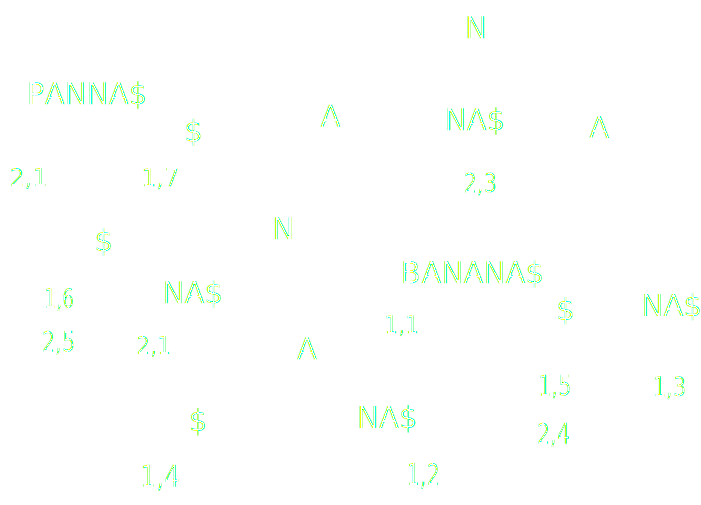
\includegraphics[width=0.8\textwidth]{ST-banana-panna}
\end{center}
$s_{1}$: BANANA\$, $s_{2}$: PANNA\$
\end{frame}


\begin{frame}[fragile]
\frametitle{Sottostringa comune più lunga}
\begin{block}{$k$ stringhe $\{s_{1}, \ldots , s_{k}\}$}
\begin{enumerate}[<+->]
\item
Suffix tree generalizzato
\item
Vettore $C_{x}[1:k]$ per ogni nodo $x$
\item
$C_{x}[i]$: sottoalbero con radice $x$ ha una foglia di $s_{i}$
\item
$C_{x} = \bigvee C$ sui figli di $C$
\item
Nodo $z$, $C_{z}=$ tutti ${1}$
\item
Tempo $O(kn)$
\item
$n$: summa lunghezze $|s_{1}| + \cdots + |s_{k}|$
\end{enumerate}
\end{block}
\end{frame}


\begin{frame}[fragile]
\frametitle{Lowest common ancestor (lca)}
\begin{block}{Dati albero $T$ e 2 foglie $x$, $y$}
\begin{itemize}
\item
$z$ è antenato comune di $x$, $y$ se
$z$ è antenato di entrambi $x$ e $y$
\item
$z$ è lca di $x$, $y$ se:
\begin{enumerate}
\item
$z$ è antenato comune di $x$ e $y$
\item
nessun discendente di $z$ è antenato comune di $x$ e $y$
\end{enumerate}
\end{itemize}
\end{block}
\begin{block}{Proprietà}
\begin{itemize}
\item
Preprocessing di $T$ in tempo $O(n)$
\item
Calcolo lca$(x,y)$ in tempo $O(1)$
\item
Algoritmo complesso, ma pratico
\end{itemize}
\end{block}
\end{frame}

\begin{frame}[fragile]
\frametitle{Sottostringa comune più lunga di $k$ stringhe}
\begin{block}{Arricchimento $ST$}
\begin{enumerate}[<+->]
\item
$N_{x}[i]$: numero foglie di $s_{i}$ discendenti di $x$
\item
$N_{x}[i]=0$ o $1$ per ogni foglia
\item
$N_{x}[i]=$ somma dei figli
\item
$D_{x}[i]$: numero di consecutive di foglie di $s_{i}$, ordinate secondo visita depth-first, discendenti di $x$
\item
$N_{x}[i]=0 \Rightarrow D_{x}[i]=0$
\item
$N_{x}[i]=1 \Rightarrow D_{x}[i]=0$
\item
$N_{x}[i]\ge 1 \Rightarrow D_{x}[i]=N_{x}[i]-1$
\item
$N_{x}[i] - D_{x}[i] =$ \uncover<2->{$C_{x}[i]$}
\end{enumerate}
\end{block}
\end{frame}

\begin{frame}[fragile]
\frametitle{Sottostringa comune più lunga di $k$ stringhe}
\begin{block}{Gestione $ST$}
\begin{itemize}
\item
Visita depth-first di $ST$
\item
$L_{i}$: lista ordinata delle foglie di $s_{i}$
\item
Per ogni coppia $x,y$ consecutiva in $L_{i}$
\begin{enumerate}
\item
$z\gets lca(x,y)$
\item
$D_{z}[i]=$
\item
Aggiorna $C_{z}$
\end{enumerate}
\end{itemize}
\end{block}
\end{frame}

\begin{frame}[fragile]
\frametitle{Allineamento di 2 sequenze}
\begin{block}{Allineamento}
\begin{itemize}
\item
Input: 2 sequenze $s_{1}$ e $s_{2}$
\item
Aggiunta di \alert{indel} in $s_{1}$ e $s_{2}$
\item
sequenze estese = stessa lunghezza
\item
NO colonne di indel
\end{itemize}
\end{block}
\end{frame}

\begin{frame}[fragile]
\frametitle{Allineamento: esempio}
\begin{block}{Input}
\texttt{ABRACADABRA}\\
\texttt{BANANA}
\end{block}

\begin{block}{sequenze allineate 1}
\texttt{ABRACADABRA}\\
\texttt{-B-ANA---NA}
\end{block}
\begin{block}{sequenze allineate 2}
\texttt{ABR-AC-ADABRA}\\
\texttt{---B-ANA---NA}
\end{block}
\begin{block}{sequenze allineate 3}
\texttt{ABRACADABRA}\\
\texttt{-BANA----NA}
\end{block}
\end{frame}

\begin{frame}[fragile]
\frametitle{Allineamento: costo o valore?}
\begin{block}{Problema di ottimizzazione}
\begin{itemize}
\item
Istanza: insieme infinito di casi
\item
Soluzioni ammissibili: ammissibilità verificabile in tempo polinomiale
\item
Funzione obiettivo: Istanza $\mapsto \mathbb{R}^{+}$
\item
Massimizzazione o minimizzazione
\end{itemize}
\end{block}
\begin{block}{costo o valore?}
\begin{itemize}
\item
Costo da minimizzare
\item
Valore da massimizzare
\end{itemize}
\end{block}
\end{frame}

\begin{frame}[fragile]
\frametitle{Valore}
\begin{block}{Valore di un allineamento}
\begin{itemize}[<+->]
\item
Somma dei valori delle singole colonne
\item
Valore di una colonna =
\item
valore in ingresso
\end{itemize}
\end{block}

\only<4->{\begin{block}{Istanza}
\begin{itemize}
\item
due sequenze $s_{1}$ e $s_{2}$
\item
matrice di score
$d:\left(\Sigma\cup\{-\}\right)\times\left(\Sigma\cup\{-\}\right) \mapsto
\mathbb{R^{+}}$
\item
problema di massimizzazione = massima omologia
\end{itemize}
\end{block}}
\end{frame}

\begin{frame}[fragile]
\frametitle{Needleman-Wunsch: Equazione di ricorrenza}
\begin{block}{Definizione}
$M[i,j] = $ ottimo su $s_{1}[:i]$, $s_{2}[:j]$
\end{block}
\begin{equation*}
M[i,j] = \max \left\{
\begin{array}{r}%{r@{\quad }l}
M[i-1, j-1] + d(s_{1}[i], s_{2}[j])\\
M[i  , j-1] + d( -     , s_{2}[j])\\
M[i-1, j  ] + d(s_{1}[i], -      )
\end{array}
\right.
\end{equation*}
\begin{block}{Condizione al contorno}
\begin{itemize}
\item
$M[0,0] = 0$
\item
$M[i,0] = M[i-1,0] + d(s_{1}[i],-)$
\item
$M[0,j] = M[0,j-1 + d(-,s_{2}[j])$
\end{itemize}
\end{block}
\end{frame}


\begin{frame}[fragile]
\frametitle{Allineamento locale}
\begin{block}{Allineamento globale}
Si allineano le sequenze intere
\end{block}
\begin{block}{Allineamento locale}
\begin{enumerate}
\item
Input: $s_{1}$, $s_{2}$, matrice di score $d$
\item
Individuare sottostringhe $t_{1}$ di $s_{1}$ e $t_{2}$ di $s_{2}$ tale che
\item
$All[t_{1}, t_{2}] \geq All[u_{1}, u_{2}]$ per ogni coppia di sottostringhe
$u_{1}, u_{2}$ di $s_{1}, s_{2}$.
\item
Algoritmo banale:
calcolo tutte le sottostringhe di $s_{1}$, $s_{2}$ e ne
calcolo allineamento globale
\item
Tempo $O(n^{3}m^{3})$
\end{enumerate}
\end{block}
\end{frame}

\begin{frame}[fragile]
\frametitle{Smith-Waterman}
\begin{block}{Osservazione 1}
\begin{enumerate}
\item
Matrice $M[i,j]$ memorizza allineamento di tutte le coppie di \alert{prefissi} di
$s_{1}$, $s_{2}$
\item
Allineamento massimo fra coppie di prefissi = valore massimo in $M$
\end{enumerate}
\end{block}
\begin{block}{Osservazione 2}
\begin{enumerate}
\item
$M[0,0] = 0$
\item
quindi non si prendono sottostringhe con allineamento negativo
\end{enumerate}
\end{block}
\end{frame}

\begin{frame}[fragile]
\frametitle{Equazione di ricorrenza}
\begin{block}{Definizione}
$M[i,j] = $ ottimo fra tutte le stringhe $s_{1}[k:i]$, $s_{2}[h:j]$
\end{block}
\begin{equation*}
M[i,j] = \max \left\{
\begin{array}{r}%{r@{\quad }l}
M[i-1, j-1] + d(s_{1}[i], s_{2}[j])\\
M[i  , j-1] + d( -     , s_{2}[j])\\
M[i-1, j  ] + d(s_{1}[i], -      )\\
0
\end{array}
\right.
\end{equation*}
\begin{block}{Condizione al contorno}
\begin{itemize}
\item
$M[0,0] = M[i,0] = M[0,j] =0$
\item
punto finale = valore massimo
\item
si risale nell'allineamento fino a uno $0$.
\item
Tempo $(nm)$
\end{itemize}
\end{block}
\end{frame}



\begin{frame}[fragile]
\frametitle{Gap}
\begin{block}{Definizione}
\begin{enumerate}
\item
Sequenza contigua di indel in un \alert{allineamento}
\end{enumerate}
\end{block}
\begin{block}{Esempio}
\texttt{ABR\alert{-}AC\alert{-}ADABRA}: 2 gap\\
\texttt{\alert{---}B\alert{-}ANA\alert{---}NA}: 3 gap
\end{block}
\begin{block}{Osservazione}
\begin{enumerate}
\item
Un gap sposta il frame di lettura
\item
1 indel $\approx$ 2 indel
\end{enumerate}
\end{block}
\end{frame}

\begin{frame}[fragile]
\frametitle{Allineamento con gap generici}
\begin{itemize}[<+->]
\item
costo gap lungo $l$: $P(l)$
\item
Come descrivo l'allineamento ottimo?
\item
Come è fatta l'ultima colonna?
\item
Come è fatto l'ultimo gap?
\end{itemize}
\end{frame}

\begin{frame}[fragile]
\frametitle{Gap generico}
\begin{block}{Definizione}
$M[i,j] = $ ottimo su $s_{1}[:i]$, $s_{2}[:j]$
\end{block}
\begin{equation*}
M[i,j] = \max \left\{
\begin{array}{r}%{r@{\quad }l}
M[i-1, j-1] + d(s_{1}[i], s_{2}[j])\only<2>{\alert{\text{ no gap}}}\\
\max_{l>0} M[i  , j-l] + P(l)\only<2>{\alert{\text{ gap in }s_{1}}}\\
\max_{l>0} M[i-l, j  ] + P(l)\only<2>{\alert{\text{ gap in }s_{2}}}
\end{array}
\right.
\end{equation*}
\begin{block}{Condizione al contorno}
\begin{itemize}[<+->]
\item
$M[0,0] = 0$
\item
$M[i,0] = P(i)$, $M[0,j] = P(j)$
\item
Tempo $O(nm(n+m))$
\end{itemize}
\end{block}
\end{frame}


\begin{frame}[fragile]
\frametitle{Allineamento con gap affine}
\begin{itemize}[<+->]
\item
costo gap lungo $l$: $P_{o} + lP_{e}$
\item
$P_{o}$: costo apertura gap
\item
$P_{e}$: costo estensione gap
\item
$P_{e}, P_{o}>0$
\item
Come descrivo l'allineamento ottimo?
\item
Come è fatta l'ultima colonna?
\item
Come è fatto l'ultimo gap?
\end{itemize}
\end{frame}


\begin{frame}[fragile]
\frametitle{Gap affine}
\begin{block}{Definizione}
\begin{itemize}
\item
$M[i,j] = $ ottimo su $s_{1}[:i]$, $s_{2}[:j]$
\item
$E_{1}[i,j] = $ ottimo su $s_{1}[:i]$, $s_{2}[:j]$, con estensione di gap finale
in $s_{1}$
\item
$E_{2}[i,j] = $ ottimo su $s_{1}[:i]$, $s_{2}[:j]$, con estensione di gap finale
in $s_{2}$
\item
$N_{1}[i,j] = $ ottimo su $s_{1}[:i]$, $s_{2}[:j]$, con apertura di gap alla
fine di $s_{1}$
\item
$N_{2}[i,j] = $ ottimo su $s_{1}[:i]$, $s_{2}[:j]$, con apertura di gap alla
fine di $s_{1}$
\end{itemize}
\end{block}
\end{frame}

\begin{frame}[fragile]
\frametitle{Gap affine}
\begin{equation*}
M[i,j] = \max \left\{
\begin{array}{l}%{r@{\quad }l}
M[i-1, j-1] + d(s_{1}[i], s_{2}[j])\\
E_{1}[i,j],
E_{2}[i,j] \\
N_{1}[i,j],
N_{2}[i,j]
\end{array}
\right.
\end{equation*}
\begin{equation*}
E_{1}[i,j] = \max \left\{
\begin{array}{l}%{r@{\quad }l}
E_{1}[i,j-1] + P_{e}\\
N_{1}[i,j-1] + P_{e}
\end{array}
\right.
\end{equation*}
\begin{equation*}
E_{2}[i,j] = \max \left\{
\begin{array}{l}%{r@{\quad }l}
E_{2}[i-1,j] + P_{e} \\
N_{2}[i-1,j] + P_{e}
\end{array}
\right.
\end{equation*}
\begin{equation*}
N_{1}[i,j] = M[i,j-1] + P_{o} + P_{e}, \quad
N_{2}[i,j] = M[i-1,j] + P_{o} + P_{e}
\end{equation*}
\end{frame}

\begin{frame}[fragile]
\frametitle{Allineamento multiplo}
\begin{block}{$k$ sequenze}
\begin{itemize}[<+->]
\item
Input: insieme di sequenze $\{s_{1}, \ldots , s_{k}\}$
\item
Aggiunta di \alert{indel} nelle sequenze
\item
sequenze estese = tutte stessa lunghezza
\item
NO colonne di indel
\end{itemize}
\end{block}
\end{frame}

\begin{frame}[fragile]
\frametitle{Valore di una colonna}
\begin{block}{SP: sum of pairs}
\begin{itemize}[<+->]
\item
$\{s_{1}, \ldots , s_{k}\} \mapsto \{s^{*}_{1}, \ldots , s^{*}_{k}\}$ allineate
\item
Valore $\{s^{*}_{1}[h], \ldots , s^{*}_{k}[h]\}$
\item
$\sum_{i<j} d(s^{*}_{1}[i], s^{*}_{k}[j])$
\end{itemize}
\end{block}
\begin{block}{Complessità}
\begin{itemize}[<+->]
\item
se $k$ è arbitrario $\Rightarrow$ NP-completo
\item
se $k$ è fissato $\Rightarrow$ tempo $O(n^{k})$
\end{itemize}
\end{block}
\end{frame}


\begin{comment}
\begin{frame}[fragile]
\frametitle{Allineamento con banda.}
\begin{enumerate}
\item
$Opt$ = valore allineamento
\end{frame}
\end{frame}

\begin{comment}
\begin{frame}[fragile]
\frametitle{Algoritmo di Carrillo-Lipman}
\begin{quote}{Euristica}
\begin{enumerate}
\item
Input: $3$ sequenze $s_{1}$, $s_{2}$, $s_{3}$
\item
Non visitiamo tutta la matrice di programmazione dinamica
\item
Caso peggiore $O(n^{3})$
\end{enumerate}
\end{quote}
\end{frame}
\end{comment}

\begin{frame}[fragile]
\frametitle{Matrici di sostituzione}
\begin{enumerate}
\item
Utilizzate per valutare un allineamento
\item
Implicitamente probabilità di transizione
\item
Mutazioni ricorrenti
\item
Allineamenti di proteine
\end{enumerate}
\end{frame}

\begin{frame}[fragile]
\frametitle{PAM: unità di misura}
\begin{enumerate}
\item
PAM: point/percent accepted mutation
\item
due sequenze $s_{1}$ e $s_{2}$: quanto sono distanti?
\item
distanza 1PAM $\Rightarrow$ numero mutazioni = $\frac{1}{100} |s_{1}|$
\item
semplice in assenza di indel
\item
Mutazioni ricorrenti $\Rightarrow$ misura affidabile solo per piccoli valori
\item
$s_{1}$ e $s_{2}$ distanti $100$ PAM $\Rightarrow$ una singola base ha 36\% di
probabilità di non essere mutata
\end{enumerate}
\end{frame}

\begin{frame}[fragile]
\frametitle{Matrici PAM}
\begin{enumerate}
\item
dipende dalla distanza attesa
\item
PAM250, PAM200, PAM1
\end{enumerate}
\begin{block}{Calcolo PAM$k$}
\begin{enumerate}
\item
Costruzione PAM$k$
\item
Si prendono varie sequenze distanti $k$PAM
\item
si allineano le sequenze
\item
si calcolano le frequenze $f(i)$, $f(i,j)$ di tutti i singoli caratteri e le
coppie di caratteri
\item
PAM$k(i,j)=\log\frac{f(i,j)}{f(i)f(j)}$
\end{enumerate}
\end{block}
\end{frame}

\begin{frame}[fragile]
\frametitle{Log odds ratio}
\begin{block}{Odds ratio}
\begin{enumerate}
\item
$\frac{p}{1-p}$, $p$ è la probabilità dell'evento interessante (target)
\item
$\frac{f(i,j)}{f(i)f(j)}$
\item
$f(i,j)$: frequenza della mutazione misurata
\item
$f(i)f(j)$: ipotesi nulla (caratteri indipendenti)
\end{enumerate}
\end{block}
\end{frame}


\begin{frame}[fragile]
\frametitle{Matrici PAM}
\begin{block}{Calcolo PAM$k$ nella realtà}
\begin{itemize}
\item
Problema: come allineare se non si conosce la matrice
\item
Allineate sequenze molto simili
\item
no indel
\item
$M_{k}(i,j)=\log\frac{f(i)M_{1}^{k}(i,j)}{f(i)f(j)}=\log\frac{M_{1}^{k}(i,j)}{f(j)}$
\item
valori moltiplicati per $10$
\item
arrotondati all'intero più vicino
\item
si somma un intero a tutti i valori
\end{itemize}
\end{block}
\end{frame}


\begin{frame}[fragile]
\frametitle{Matrici BLOSUM}
\begin{block}{Confronto con PAM}
\begin{itemize}
\item
PAM allinea sequenze vicine
\item
ma viene usata per allineare sequenze lontane
\item
regioni conservate e non conservate hanno stessa importanza
\end{itemize}
\end{block}

\begin{block}{BLOCKS}
\begin{itemize}
\item
blocchi di regioni conservate
\item
scelte ``a mano''
\item
$B(i,j)=\log\frac{f(i,j)}{f(i)f(j)}$
\end{itemize}
\end{block}
\end{frame}

\begin{frame}[fragile]
\frametitle{Matrici BLOSUM}
\begin{block}{BLOSUM$x$}
\begin{itemize}
\item
le sequenze che sono simili più di $x$\% vengono clusterizzate
\item
cluster = rimuovere tutte tranne una
\item
scopo:  evitare di sovrapesare parti sovrarappresentate nel campione
\item
BLOSUM62: più usata per gli allineamenti
\end{itemize}
\end{block}
\end{frame}


\begin{frame}[fragile]
\frametitle{Statistiche Karlin-Altschul}
\begin{block}{Ricerca in un database}
\begin{itemize}
\item
Punteggio positivo possibile
\item
Punteggio medio negativo
\item
Simboli indipendenti e equiprobabili
\item
Sequenze infinitamente lunghe
\item
Allineamenti senza gap
\end{itemize}
\end{block}
\end{frame}

\begin{frame}[fragile]
\frametitle{Equazione Karlin-Altschul}
\begin{equation*}
E=kmne^{-\lambda S}
\end{equation*}
\begin{itemize}
\item
$E$: numero allineamenti
\item
$k$: costante
\item
$n$: numero caratteri in database
\item
$m$: lunghezza stringa query
\item
$\lambda S$: punteggio normalizzato
\end{itemize}
\end{frame}

\begin{frame}[fragile]
\frametitle{BLAST}
\begin{block}{Basic Local Alignment Search Tool}
\begin{itemize}
\item
Ricerca seed
\item
seed = pattern matching con sottostringa di lunghezza $3$
\item
Costruzione  high-scoring segment pair (HSP)
= estensione seed
\item
Filtro seed tenuti solo HSP con  alta significatività
\item
Fusione HSP  vicine
\item
Smith-Waterman sulle regioni
\end{itemize}
\end{block}
\end{frame}


\begin{comment}
\begin{frame}[fragile]
\frametitle{BWA-SW}
\end{frame}
\end{comment}


\begin{frame}[fragile]
\frametitle{SamTools: sloccount}
\begin{verbatim}
SLOC  Directory	SLOC-by-Language (Sorted)
14688 top_dir   ansic=14688
5334  misc      perl=2777,ansic=2258,java=158,python=141
4601  bcftools  ansic=4080,perl=521
1527  win32     ansic=1527
178   examples  ansic=178

Totals grouped by language (dominant language first):
ansic:        22731 (86.34%)
perl:          3298 (12.53%)
java:           158 (0.60%)
python:         141 (0.54%)

Development Effort Estimate, Person-Years = 6.20
\end{verbatim}
\end{frame}


\begin{frame}[fragile]
\frametitle{SamTools: close file}
\lstinputlisting{code/samtools/samclose.c}
\end{frame}

\begin{frame}[fragile]
\frametitle{SamTools: read file}
\lstinputlisting{code/samtools/samread.c}
\end{frame}
\begin{frame}[fragile]
\frametitle{SamTools: write file}
\lstinputlisting{code/samtools/samwrite.c}
\end{frame}

\begin{frame}[fragile]
\frametitle{SamTools: read file}
\lstinputlisting{code/samtools/samopen1.c}
\end{frame}
\begin{frame}[fragile]
\frametitle{SamTools: read file}
\lstinputlisting{code/samtools/samopen2.c}
\end{frame}
\begin{frame}[fragile]
\frametitle{SamTools: read file}
\lstinputlisting{code/samtools/samopen3.c}
\end{frame}
\begin{frame}[fragile]
\frametitle{SamTools: read file}
\lstinputlisting{code/samtools/samopen4.c}
\end{frame}
\begin{frame}[fragile]
\frametitle{SamTools: read SAM file}
\lstinputlisting{code/samtools/samopen5.c}
\end{frame}


\begin{frame}[fragile]
\frametitle{SamTools: SAM header parse}
\lstinputlisting{code/samtools/bam_import_sam_header_parse.c}
\end{frame}

\begin{frame}[fragile]
\frametitle{SamTools: SAM header parse2}
\lstinputlisting{code/samtools/sam_import_sam_header_parse2.c}
\end{frame}


\begin{frame}[fragile]
\frametitle{SamTools: list append to end}
\lstinputlisting{code/samtools/sam_header_list_append_to_end.c}

Come è fatto \verb+list_t+?
\end{frame}


\begin{frame}[fragile]
\frametitle{SamTools: list append to end}
\lstinputlisting{code/samtools/sam_header_HeaderList.c}
\end{frame}





\begin{frame}[fragile]
\frametitle{SamTools: calDepth.c}
\lstinputlisting{code/samtools/calDepth.c}
\end{frame}
\begin{frame}[fragile]
\frametitle{SamTools: calDepth.c}
\lstinputlisting{code/samtools/calDepth-main1.c}
\end{frame}
\begin{frame}[fragile]
\frametitle{SamTools: calDepth.c}
\lstinputlisting{code/samtools/calDepth-main2.c}
\end{frame}
\begin{frame}[fragile]
\frametitle{SamTools: calDepth.c}
\lstinputlisting{code/samtools/calDepth-main3.c}
\end{frame}

\begin{frame}[fragile]
\frametitle{SamTools: bam parse region}
\lstinputlisting{code/samtools/bam_parse_region.c}
\end{frame}
\begin{frame}[fragile]
\frametitle{SamTools: bam parse region}
\lstinputlisting{code/samtools/bam_parse_region-1.c}
\end{frame}
\begin{frame}[fragile]
\frametitle{SamTools: bam parse region}
\lstinputlisting{code/samtools/bam_parse_region-2.c}
\end{frame}
\begin{frame}[fragile]
\frametitle{SamTools: bam parse region}
\lstinputlisting{code/samtools/bam_parse_region-4.c}
\end{frame}


\begin{frame}[fragile]
\frametitle{SamTools: bgzf}
\lstinputlisting{code/samtools/bgzf-1.c}
\end{frame}
\begin{frame}[fragile]
\frametitle{SamTools: bgzf}
\lstinputlisting{code/samtools/bgzf-2.c}
\end{frame}
\begin{frame}[fragile]
\frametitle{SamTools: bgzf}
\lstinputlisting{code/samtools/bgzf-3.c}
\end{frame}
\begin{frame}[fragile]
\frametitle{SamTools: bgzf}
\lstinputlisting{code/samtools/bgzf-4.c}
\end{frame}
\begin{frame}[fragile]
\frametitle{SamTools: bgzf}
\lstinputlisting{code/samtools/bgzf-5.c}
\end{frame}
\begin{frame}[fragile]
\frametitle{SamTools: bgzf}
\lstinputlisting{code/samtools/bgzf-6.c}
\end{frame}
\begin{frame}[fragile]
\frametitle{SamTools: bgzf}
\lstinputlisting{code/samtools/bgzf-7.c}
\end{frame}
\begin{frame}[fragile]
\frametitle{SamTools: bgzf}
\lstinputlisting{code/samtools/bgzf-8.c}
\end{frame}
\begin{frame}[fragile]
\frametitle{SamTools: bgzf}
\lstinputlisting{code/samtools/bgzf-9.c}
\end{frame}
\begin{frame}[fragile]
\frametitle{SamTools: bgzf}
\lstinputlisting{code/samtools/bgzf-10.c}
\end{frame}
\begin{frame}[fragile]
\frametitle{SamTools: bgzf}
\lstinputlisting{code/samtools/bgzf-11.c}
\end{frame}
\begin{frame}[fragile]
\frametitle{SamTools: bgzf}
\lstinputlisting{code/samtools/bgzf-12.c}
\end{frame}
\begin{frame}[fragile]
\frametitle{SamTools: bgzf}
\lstinputlisting{code/samtools/bgzf-13.c}
\end{frame}



\begin{frame}[fragile]
\frametitle{Filogenesi. Neighbor-Joining.}
\end{frame}

\begin{frame}[fragile]
\frametitle{Clearcut}
\end{frame}

\begin{frame}[fragile]
\frametitle{Sequenziamento e grafi di de Brujin}
\end{frame}

\begin{frame}[fragile]
\frametitle{Velvet}
\end{frame}



\begin{comment}
\begin{frame}[fragile]
\frametitle{SAIS}
\lstinputlisting{code/sais/sais.c}
\end{frame}


\begin{frame}[fragile]
\frametitle{SAIS}
\lstinputlisting{code/sais/sais_main.1}
\end{frame}
\end{comment}


%  \begin{frame}
%    \frametitle{Consensus Clustering}
%    \begin{block}{Problem}
%      \alert{Input}: set $\Pi$ of partitions of $U$\\
%      \alert{Output}: a partition $P$ of $U$\\
%      \alert{Goal}: $P$ the best possible representative of $\Pi$
%    \end{block}

%    \begin{block}{Objective Function}
%      \begin{itemize}
%      \item
%        Symmetric difference between two partitions =
%        Pairs of elements clustered differently
%      \item
%        $d(P,\Pi)=\sum_{\pi\in \Pi}d(\pi,P)$
%      \end{itemize}
%    \end{block}
%  \end{frame}



% \begin{frame}\frametitle{Finestre}
%   \begin{itemize}
%   \item
%     Editor (F5)
%   \item
%     Log (F6)
%   \item
%     Output (F7)
%   \item
%     Icona Esegui (F8)
%   \end{itemize}
% \end{frame}




\begin{frame}[containsverbatim]\frametitle{Licenza d'uso}
  \small

  Quest'opera {\`e} soggetta alla licenza Creative Commons: Attribuzione-Condividi
  allo stesso modo 3.0.

  \verb+http://creativecommons.org/licenses/by-sa/3.0/+

  Sei libero di riprodurre, distribuire, comunicare al pubblico, esporre in
  pubblico, rappresentare, eseguire, recitare e modificare quest'opera
  alle seguenti condizioni:
  \begin{itemize}
  \item
    Attribuzione — Devi attribuire la paternit{\`a} dell'opera nei modi indicati
    dall'autore o da chi ti ha dato l'opera in licenza e in modo tale da non
    suggerire che essi avallino te o il modo in cui tu usi l'opera.
  \item
    Condividi allo stesso modo — Se alteri o trasformi quest'opera, o se la usi
    per crearne un'altra, puoi distribuire l'opera risultante solo con una licenza
    identica o equivalente a  questa.
  \end{itemize}
  \vspace*{1cm}
\end{frame}



\begin{comment}
\begin{frame}[fragile]
\frametitle{SAIS}
\begin{block}{S-type/L-type suffix}
\begin{itemize}
\item
$S[i:]$ e $S[i]$ sono  S-type se $S[i:] < S[i+1:]$
\item
$S[i:]$ e $S[i]$ sono  L-type se $S[i:] > S[i+1:]$
\item
$S[n-1:]$ è S-type
\end{itemize}
\end{block}

\begin{block}{Test S-type}
$S[i]$ è S-type se:
\begin{enumerate}
\item
$S[i] < S[i + 1]$ oppure
\item
$S[i] = S[i + 1]$ e  $S[i + 1]$ sono S-type
\end{enumerate}
\end{block}
\end{frame}

\begin{frame}[fragile]
\frametitle{SAIS}
\begin{block}{Bucket}
Sottoarray dei suffissi che iniziano con lo stesso carattere
\end{block}
\begin{block}{S-type/L-type Bucket}
\begin{enumerate}
\item
All'interno di un bucket,  L-suffissi precedono S-suffissi
\item
L-bucket, S-bucket
\end{enumerate}
\end{block}
\end{frame}

\begin{frame}[fragile]
\frametitle{SAIS}
\alert{LMS}: Leftmost S-type
\begin{block}{LMS character}
$S[i]$ è LMS se $S[i]$ è S-type e $S[i-1]$ è L-type
\end{block}
\begin{block}{LMS suffix}
$S[i:]$ è LMS se $S[i]$ è LMS
\end{block}
\begin{block}{LMS substring}
\begin{itemize}
\item
$S[n-1:n-1]$ è LMS
\item
$S[i:j]$ è LMS se $S[i]$ e $S[j]$ sono LMS e nessun $S[l]$ con $i<l<j$ è LMS
\end{itemize}
\end{block}
\end{frame}


\begin{frame}[fragile]
\frametitle{SAIS: sais.h}
\lstinputlisting{code/sais/sais.h}
\begin{block}{Parametri}
\begin{itemize}
\item
\verb!k!: dimensione alfabeto
\item
\verb!n!: lunghezza testo
\item
\verb!T!: Testo
\item
\verb!SA!: Suffix Array
\end{itemize}
\end{block}
\end{frame}

\begin{frame}[fragile]
\frametitle{SAIS: main}
\lstinputlisting{code/sais/sais_int.c}
\onslide<2->{\lstinline+sais_main+ gestisce i casi non banali}
\end{frame}




\begin{frame}[fragile]
\frametitle{SAIS}
\lstinputlisting{code/sais/sais.C-alphabet.c}
\end{frame}

\begin{frame}[fragile]
\frametitle{SAIS}
\lstinputlisting{code/sais/sais.start-end-bucket.c}
  \begin{itemize}[<+->]
  \item
Come migliorare il codice?
\item
12: \lstinline!B[i]=sum; sum+=C[i];!
\end{itemize}
\end{frame}


\begin{frame}[fragile]
\frametitle{SAIS: sais\_main}
\lstinputlisting{code/sais/sais_main.1}
code/sais/sais.c
\end{frame}


\begin{frame}[fragile]
\frametitle{SAIS: sais\_main}
\lstinputlisting{code/sais/sais_main.2}
\end{frame}


\begin{frame}[fragile]
\frametitle{SAIS: sais\_main}
\lstinputlisting{code/sais/sais_main.2.1}
\end{frame}


\begin{frame}[fragile]
\frametitle{SAIS: sais\_main}
\lstinputlisting{code/sais/sais_main.3}
\end{frame}
\end{comment}


\end{document}
%%% Local Variables:
%%% TeX-PDF-mode: t
%%% TeX-master: "lucidi_bioinformatica_video"
%%% buffer-file-coding-system: utf-8
%%% End:
